% Part: sets-functions-relations
% Chapter: relations
% Section: trees

\documentclass[../../../include/open-logic-section]{subfiles}

\begin{document}

\olfileid[tr]{sfr}{rel}{tre}
\olsection{Ağaçlar}

Mantığın bütün alanlarında önemli bir rol oynayan özel bir kısmi sıralama türü
\emph{ağaçtır}. Sonlu ağaçlar mantığın temel bölümlerinde karşımıza çıkar:
örneğin formüller, bir sözdizim ağacına ayrıştırılmaları aracılığıyla
anlaşılabilir; birçok türetim sistemindeki türetimler de sonlu ağaç biçimini
alır.
%
Sonsuz ağaçlar, önerme mantığı ile birinci dereceden mantığın tamlık
teoremlerinin ispatlarında bile ortaya çıkar ve matematiksel mantığın
her yanında kullanılır.

Küme kuramsal ağaç kavramı, çizge kuramındaki ağaç kavramıyla yakından
ilişkilidir. Aşağıda (sonlu) bir ağacın resmi vardır:

\begin{center}
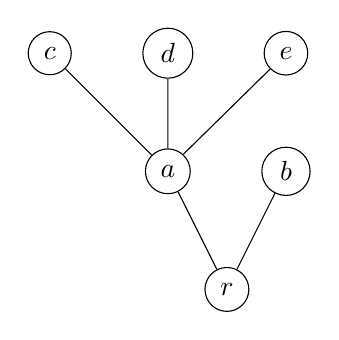
\begin{tikzpicture}[nodes={draw, circle}, -]
\node{$r$} [grow'=up]
    child { node {$a$}
        child { node {$c$} }
        child { node {$d$} }
        child { node {$e$} }
    }
    child { node {$b$} };
\end{tikzpicture}
\end{center}

En alttaki düğüm~$r$ köktür. $r$ dışındaki her düğümün hemen altında tam
olarak bir ebeveyn düğüm vardır. Kenarlar yukarı doğru izlenerek $x$
düğümünden $y$ düğümüne ulaşılabiliyorsa, $x$'in $y$ ile kurduğu bağıntıyı
$x$'in $y$'nin \emph{atası} olması biçiminde düşünebiliriz.

Bir ağaçtaki ata bağıntısı sıkı bir kısmi sıralamadır. Küme kuramsal tanımın
güdüsü budur. Tanımı vermek için iki kavrama gereksinimimiz vardır. $\le$ ile
kısmi sıralanmış bir $A$ kümesindeki \emph{en küçük eleman}, bütün $y \in A$
için $x \le y$ olan bir $x \in A$ elemanıdır. Boş olmayan her alt kümesinin en
küçük bir elemanı varsa bir küme $\le$ ile \emph{iyi sıralanmıştır}.

\begin{defn}[Ağaç]
Bir \emph{ağaç}, $T=\tuple{A,\le}$ ikilisidir; burada $A$ bir kümedir ve
$\le$, $A$ üzerinde benzersiz bir en küçük $r \in A$ elemanına (\emph{kök}
denir) sahip öyle bir kısmi sıralamadır ki her $x \in A$ için
$\Setabs{y}{y \le x}$ kümesi $\le$ ile iyi sıralanmıştır.
\end{defn}

\begin{defn}[Ardıllar]
$T=\tuple{A,\le}$ bir ağaç olsun. $x,y \in A$, $x<y$ ve $x<z<y$ olacak
biçimde hiçbir $z \in A$ yoksa $y$'ye $x$'in bir \emph{ardılı} deriz.
\end{defn}

$x \in A$ elemanının ardıllarına onun \emph{çocukları} da denir. $y$, $x$'in bir
ardılıysa $x$'e $y$'nin \emph{öncülü} veya \emph{ebeveyni} deriz.

\begin{prop}
$\tuple{A,\le}$ bir ağaçsa kök dışındaki her $x \in A$ elemanının en fazla bir
öncülü vardır.
\end{prop}

\begin{proof}
  $y_1<x$, $y_2<x$ ve $y_1\neq y_2$ olduğunu varsayalım. O zaman
  $\{y_1,y_2\}\subseteq\Setabs{z}{z<x}$. $\Setabs{z}{z<x}$ kümesi $\le$ ile
  iyi sıralandığından, onun $\{y_1,y_2\}$ alt kümesinin en küçük bir elemanı
  vardır; bu eleman açıkça ya $y_1$ ya da~$y_2$ olmalıdır. Dolayısıyla ya
  $y_1\le y_2$ ya da $y_2\le y_1$. $y_1\neq y_2$ varsayımından aslında ya
  $y_1<y_2$ ya da $y_2<y_1$ sonucu çıkar. Ayrıca $y_1<x$ ve $y_2<x$
  varsayımlarından ya $y_1<y_2<x$ ya da $y_2<y_1<x$ olur. Dolayısıyla $y_1$
  ile $y_2$'nin ikisi birden $x$'in öncülü olamaz.
\end{proof}

\begin{defn}
Bir $T=\tuple{A,\le}$ ağacına, $A$ sonsuz bir kümeyse \emph{sonsuz}; değilse
\emph{sonlu} denir. $T$'de her $x \in A$ elemanının yalnızca sonlu sayıda ardılı
varsa $T$'ye \emph{sonlu dallanan} deriz.
\end{defn}

\begin{defn}[Dallar]
Bir $T=\tuple{A,\le}$ ağacı verildiğinde, $T$'nin bir \emph{dalı} $T$'deki
maksimal bir zincirdir; yani bütün $x,y \in B$ için ya $x\le y$ ya da
$y\le x$ olacak ve her $z \in A\setminus B$ için ne $z\le u$ ne de $u\le z$
olacak biçimde bir $u \in B$ bulunacak şekilde bir $B \subseteq A$ kümesidir.
%
$T$'nin bütün dallarının kümesini $[T]$ ile gösteririz.
\end{defn}

\begin{ex}
Sonlu dallanan bir ağacın klasik örneği, $0$ ve~$1$'lerden oluşan sonlu
dizilerin \emph{sonsuz ikili ağacı}dır. Bu ağaç kimi zaman $\{0,1\}^*$ ya
da~$\Bin^*$ ile gösterilir ve uzantı bağıntısı $\sqsubseteq$ ile sıralanır
(örneğin $101 \sqsubseteq 101101$). Her ikili dize, sonuna bir $0$ ya da $1$
eklenerek her zaman uzatılabildiği için bu ağaç sonsuz sayıda eleman içerir:
her $s$ elemanının tam olarak iki ardılı, $s0$ ve~$s1$ vardır. Ağacın kökü boş
dizi $\emptyseq$'dir.
\end{ex}

\begin{ex}
Biraz daha genel olarak, doğal sayıların sonlu dizileri kümesi $\Nat^*$ da
uzantı bağıntısı~$\sqsubseteq$ ile bir ağaçtır. Açıkça sonlu dallanan değildir:
her $s \in \Nat^*$, her $n \in \Nat$ için bir tane olmak üzere sonsuz sayıda
$sn$ ardılına sahiptir. $\sqsubseteq$ altında kapalı olan her
$A \subseteq \Nat^*$, $\Nat^*$'ın bir \emph{alt ağacıdır}. (Yani $A$ öyledir
ki $s \in A$ ve $s' \sqsubseteq s$ ise $s' \in A$ da olur.) Bütün sonlu
ağaçlar $\Nat^*$'ın sonlu alt ağaçları olarak temsil edilebilir.
\end{ex}

\begin{prop}[K\H{o}nig lemması]
$T=\tuple{A,\le}$ sonlu dallanan sonsuz bir ağaçsa $T$'nin sonsuz bir dalı
vardır.
\end{prop}

K\H{o}nig lemmasının hesaplanabilirlik teorisinde yaygın biçimde kullanılan ve
\emph{zayıf K\H{o}nig lemması} olarak bilinen özel bir durumu şudur:
$\{0,1\}^*$'ın her sonsuz alt ağacının sonsuz bir dalı vardır.

\end{document}
